\documentclass[]{extarticle}

\usepackage[utf8]{inputenc}
\usepackage[english]{babel}
\usepackage{hyperref}
\usepackage{extsizes}
\usepackage{caption}
\usepackage{subcaption}
\usepackage[table,dvipsnames]{xcolor}
\definecolor{lgray}{gray}{0.95}

\usepackage[square,numbers]{natbib}
\bibliographystyle{plainnat}
\setcitestyle{authoryear,open={(},close={)}}

\usepackage{amsfonts, amsmath, amssymb, amsthm}

\newtheorem{theorem}{Theorem}[section]

\usepackage{graphicx}
\usepackage{float}

\usepackage[margin=0.75in, left = 0.5in, right = 0.5in]{geometry}

\usepackage[utf8]{inputenc}
\usepackage{fancyhdr}
 
\pagestyle{fancy}
\fancyhf{}


\renewcommand{\headrulewidth}{1.5pt}% 2pt header rule
\renewcommand{\headrule}{\hbox to\headwidth{%
		\color{MidnightBlue}\leaders\hrule height \headrulewidth\hfill}}
\renewcommand{\footrulewidth}{0pt}% No footer rule
%\renewcommand{\footrule}{\hbox to\headwidth{%
%		\color{MidnightBlue}\leaders\hrule height \footrulewidth\hfill}}


\rhead{Benjamin Cox}
\chead{Statistical Consultancy -- Assessment 2}
\lhead{Due 22nd November}
\cfoot{Page \thepage}

\begin{document}

\section{Introduction}

We consider data on the survival of passengers of the RMS Titanic. The data contains many variables about the passengers of the Titanic, some of which we will use and some of which we will not. We are going to perform logistic regression in order to ascertain the effect that certain variables have on the survival of a passenger. We have 1309 individual passenger records to analyse. 

We are particularly interested in the affect of socio-economic status on survival probabilities, as well whether the adage of `women and children first' holds.

\section{Statistical Analysis}

\subsection{Introduction to our data}

The survival variable is binary (they either survived or died). This is the reason for using simple logistic regression. The passenger class is a factor variable with three levels corresponding to 1st, 2nd, and 3rd class. The sex is a factor variable with two levels corresponding to male and female. The age is a continuous variable (with rounding applied). We have data on the sum number of siblings and spouses aboard of a passenger, as well as of the number of parents and children. These are highly correlated, so we will only use one. In our case we will use the siblings and spouses. We have the ticket number, which is useless for our analysis. We have the fare paid by the passenger. This is continuous and has properties that warrant a discussion later. We have the cabin number, which we will use to ascertain whether a passenger had a cabin (this is highly correlated with passenger class). We have the port of embarkation, which is one of Cherbourg, Queenstown, and Southampton. We have the lifeboat number, which is useless, as well as the body number. These are both useless as they are a posteriori of the survival. We also have the home/destination of the passenger. This is also useless.

This time around our data has no missingness that is not appropriate. Moreover none of the variables that we are analysing have missingness (the NA in cabin number means that the passenger did not have a cabin). 

\subsection{Initial Analysis}

We first need to conduct an analysis of the independence of the variables we think we may include in our model. Performing a chi squared test we find that most variables of interest for the model are highly interdependent. However the type of model that we are fitting is somewhat resilient to this. What is important is that the variables are not co-linear. Most of our variables cannot be co-linear as they are factor variables. The only ones of concern are the sum number of siblings and spouses and the sum number of parents and children. We calculate the variance inflation factors for these variables. They come out as 1.24 and 1.23 respectively. The standard threshold for multicollinearity is 3, so we are very safe.

Looking at the fare paid by the passenger it is clear that in our data the fare paid is that of the ticket purchase, not per person. This means that those travelling in large groups will seem to pay a very large fare, whilst in reality no paying quite so high a price. Couple this with the fact that the fare is inextricably linked with both the passenger class and whether the passenger received a cabin and we are safe to remove this factor from our model. 

We will also note that there are some mistakes in the data; some ages are recorded incorrectly. As there are thousands of records we hope that the correct values will swamp the effect of the incorrect values. No attempt will be made to fix the data, as there is no reasonable way to do so in the time-frame given for this analysis.

\subsection{Model Comparison and Selection}
 First we example the independence of our variables. We do this using the $\chi^2$ test, the results of which are given in Table \ref{tab:chi}. We see that many of the variables are interdependent, which will influence our results. We see that the age, type, and floor area of a property are highly related, which is what we expected. We regress the square root of the gas consumption on all of the predictors to obtain our full model. The diagnostic plots are given in Figure \ref{fig:fmdiag}. These plots are sufficient to make general predictions.

We will now compare the full model to two sub-models. The sub-models regress gas consumption on either the base property (age, type, floor area) and on modifications to the property (loft insulation, cavity wall insulation, new boiler). The diagnostic plots are given in Figure \ref{fig:smdiag}. The plots show that both are valid models which give similar results to the initial model. We compare them to the initial model using an ANOVA test. We see that the modifications model is significantly different from the initial model, so the base properties of the property have significant effects. The property model is not statistically significantly different from the full model.  We compare the residual sum of squares (lower is better) and see that the full model has an RSS of 1244518, the property model has an RSS of 1248346, and that the modification model has an RSS of 1880124. The modifications to the property have a significantly lesser effect on the consumption than the properties inherent to the property. Looking at the Q-Q plot for the modification model one may think it is a better model. This is false; the Q-Q plot looks this way as the model is unable to predict the values that are more common and thus distort the plot. 

We choose to use the full model for our analysis as we wish to see the effects of the modifications on the property, as these are measures that can be taken after a property is constructed. The regression coefficients are given in Table \ref{tab:fulmo}. These are the expected difference in root gas consumption from the `baseline' of a property with given characteristics.

\section{Discussion of Results}

We are discussing the effect of the different variables on the square root of the gas consumption. The `baseline' results (as given in Table \ref{tab:fulmo}) are for a Bungalow in age band 1, in floor area band 1, with loft insulation greater than 150mm, without cavity walls, and without a new boiler. The predicted square root of consumption for this property is 103.7. If for example we had a semi-detached house, with a new boiler, no cavity walls, more than 150mm of loft insulation, with floor area 3, in age band 3 then our new predicted root consumption would be $$103.68 - 3.58 \text{(age)} + 0.75 \text{(semi-detached)} + 30.27 \text{(floor area)} - 2.78 \text{(New boiler)} = 128.34 \text{ root units}.$$

It must be noted that these numbers cannot be taken independently of one another: all factors must be accounted for for the model to be remotely valid. This means that one cannot say that all flats are more efficient than all bungalows: one must specify the configuration of each to make a comparison.

\subsection{Effect of Age}
We see that age has less of an effect than might be expected. The first four age bands have minimal effect. The fifth and the sixth age bands have more significant differences, with a decrease on average of 7.84 and 13.76 respectively. This means that new builds have decreased gas consumption. This may be due to the types of property built in new builds, as in Table \ref{tab:chi} we see that they are not independent.

\subsection{Effect of Type}
We see that the type of property is very significant in determining the gas consumption. Detached houses have an increased root gas consumption compared to bungalows, consuming 12.7 root units more. Semi detached consume only very slightly more, to the point that it is not significant (it is less than the standard error of the estimate). Terraced and end of terrace houses consume less. Flats consume significantly less, with 22.9 less root units on average, corresponding to 525 units less on average. 

\subsection{Effect of Floor Area}
We see that floor area has a significant effect on the gas consumption. All of them are significantly different from each other. The largest floor area consumes on average 52.56 root units, or 2762 units on average more than the smallest floor area. This is also not independent of the type of property, so we must know that changing one should have an effect on the other (ie a property with a large floor area is less likely to be a flat than detached).

\subsection{Effects of Modifications to The Property}
These effects are smaller, so will be discussed in conjunction. First we note that we see in Table \ref{tab:chi} that all of the modifications are largely independent of each other. This meshes with what we expect. We see that a new boiler decreases root gas consumption by 2.78, corresponding to an average decrease in consumption of 7.71 units. Adding cavity wall insulation has no appreciable average effect on gas consumption. Adding loft insulation above 150mm decreases root gas consumption on average by 1.98 units, corresponding to an average decrease of 3.90 units of gas consumption. We see that the standard error is equal to the estimate, so we can only really be sure that it has a small positive effect on average, and not the exact value of that effect.

\section{Conclusions}

We can conclude that if we want to decrease gas consumption we should build small flats with good insulation (loft and cavity wall) and new models of boiler. This is a foregone conclusion, but we now have numbers to back it up. A modern flat (age band 6, floor band 1) consumes 6000 fewer kWh per annum on average than an average house (mid-terrace, age band 4, floor band 2, no cavity wall, bad loft insulation, old boiler). This is a saving of approximately \pounds 230 per year (UK average price per kWh of gas is 3.8p). 

We cannot make any inferences as to why these changes make an effect from the model; the model only tells us the effect that they have. In this case it is somewhat obvious as to why the variables have the effects that they do, but it is often not. For example, flats are likely more efficient as they benefit from a collective heating effect in which flats are warmed by others around them. This is not present in detached houses. We know this from common sense, but this is not explicitly reflected in the model. 
%\pagebreak
%\bibliography{references}

\appendix

\section{Plots and Figures}

\begin{figure}[H]
	\centering
%	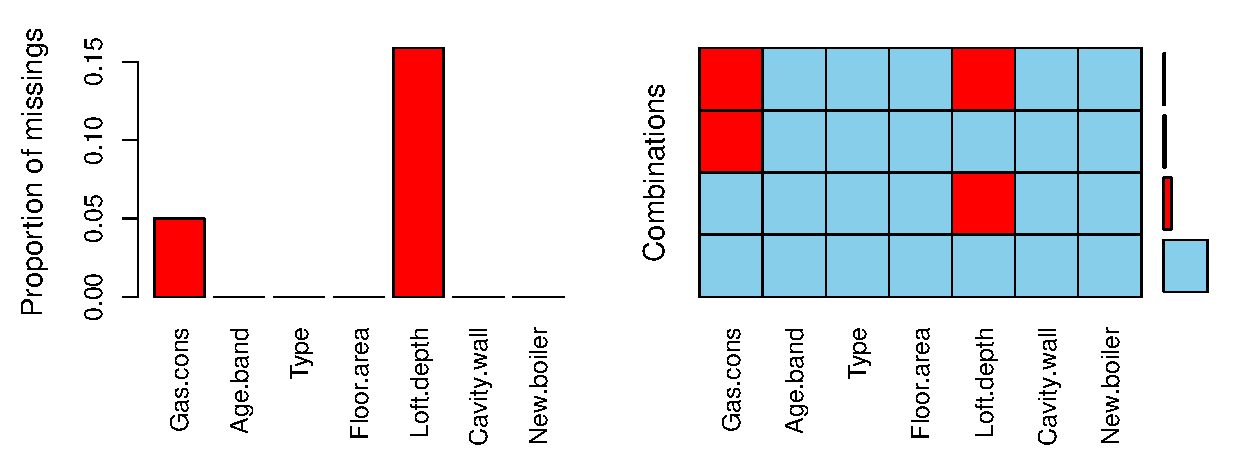
\includegraphics[width=0.7\textwidth]{aggr_missplot}
	\caption{Aggregate plot of missingness in our data}
	\label{fig:aggrmiss}
\end{figure}

\begin{figure}[H]
	\centering
%	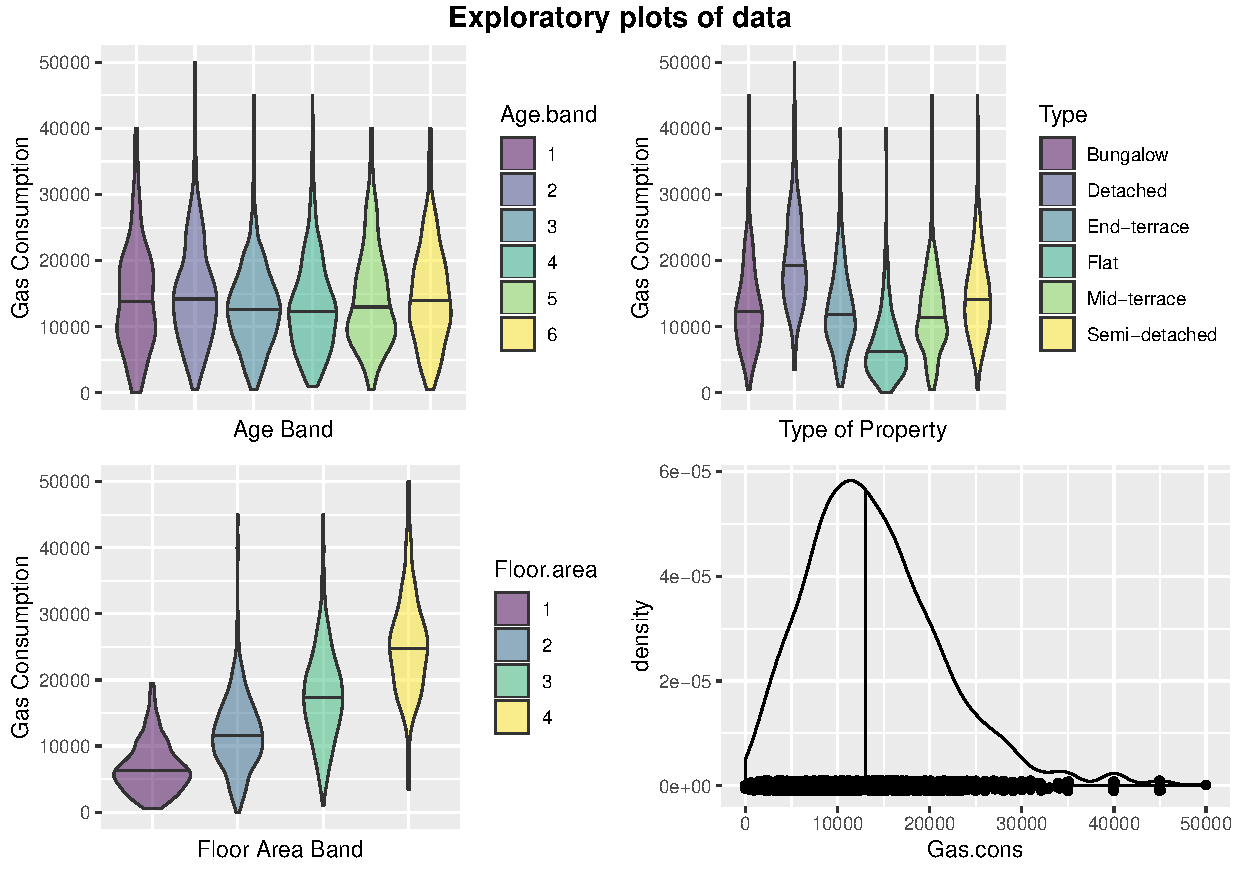
\includegraphics[width=0.7\textwidth]{datavis}
	\caption{Visualisation of data relating to gas consumption}
	\label{fig:datavis}
\end{figure}


\begin{figure}[H]
	\centering
%	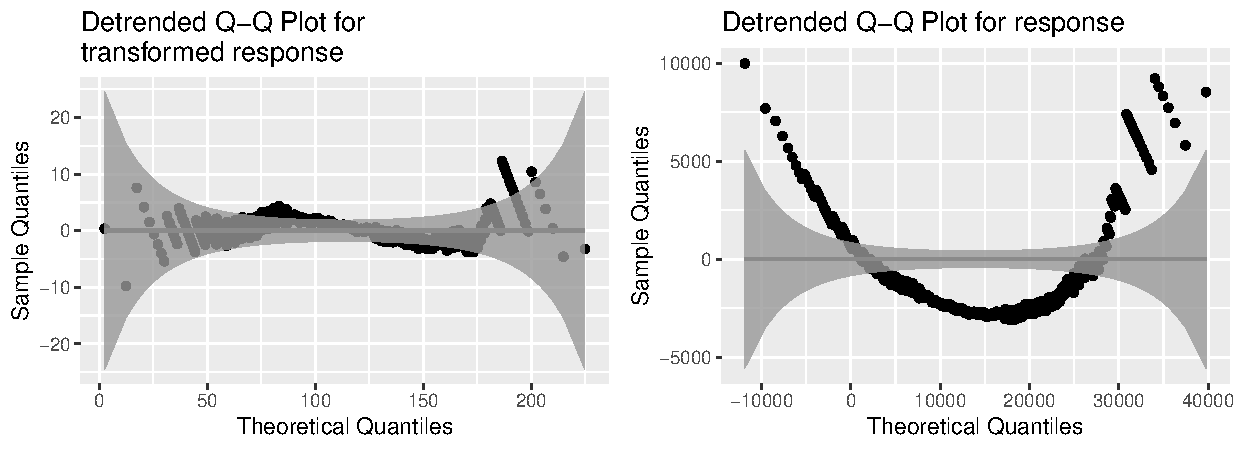
\includegraphics[width=0.7\textwidth]{qqplots}
	\caption{Model Q-Q plots for the transformed and non-transformed models}
	\label{fig:qqplots}
\end{figure}

\begin{figure}[H]
	\centering
%	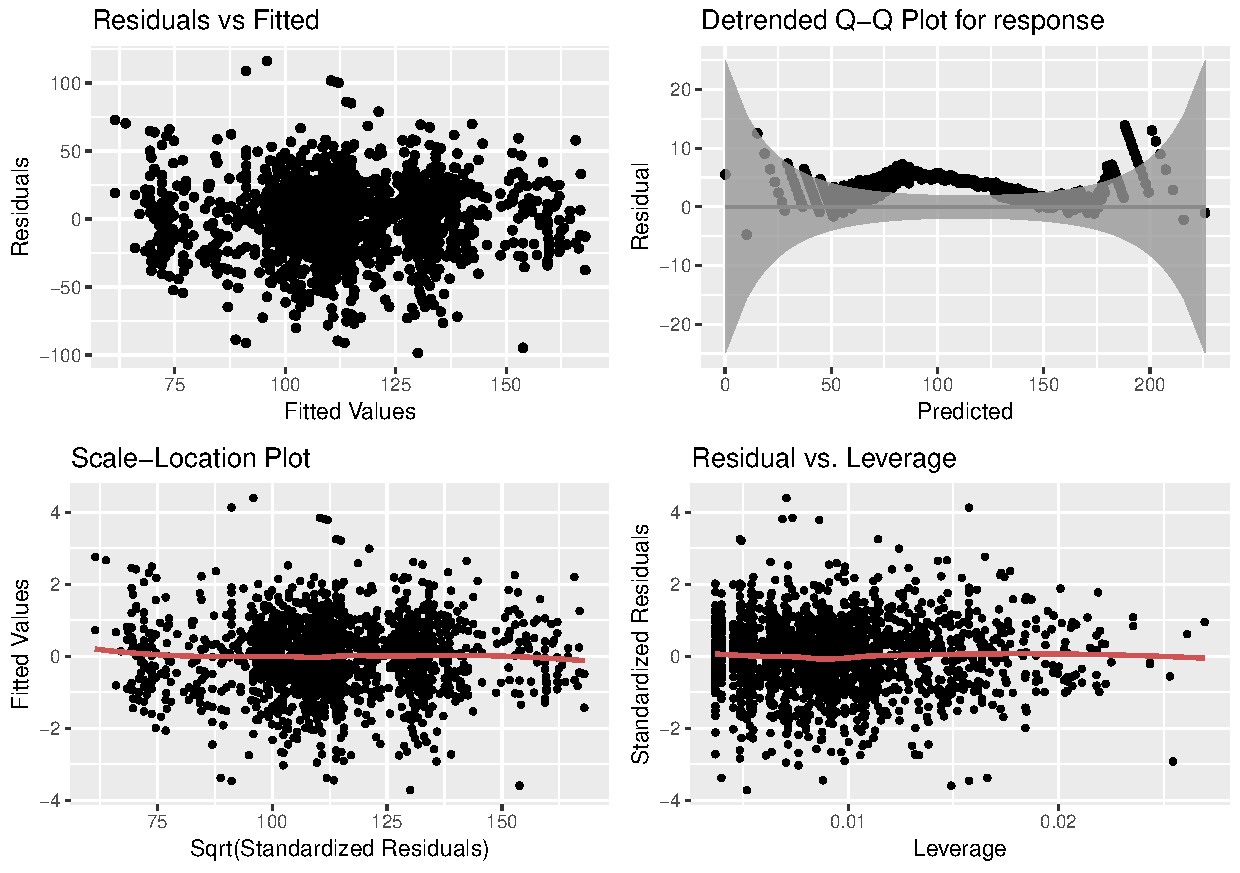
\includegraphics[width=0.7\textwidth]{fm_diag}
	\caption{Model diagnostic plots for our full model}
	\label{fig:fmdiag}
\end{figure}

\begin{figure}[H]
	\centering
%	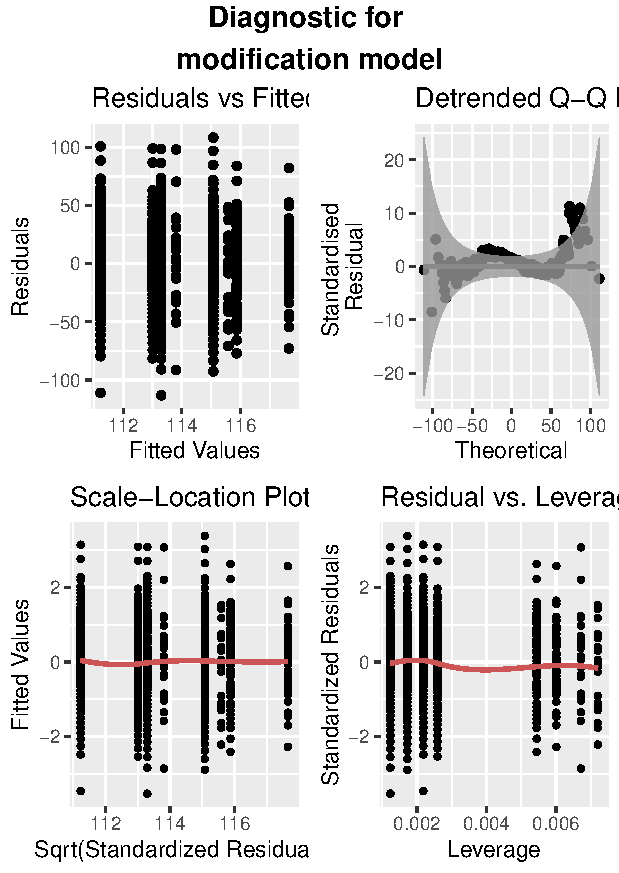
\includegraphics[width=0.4\textwidth]{diag_modif}
%	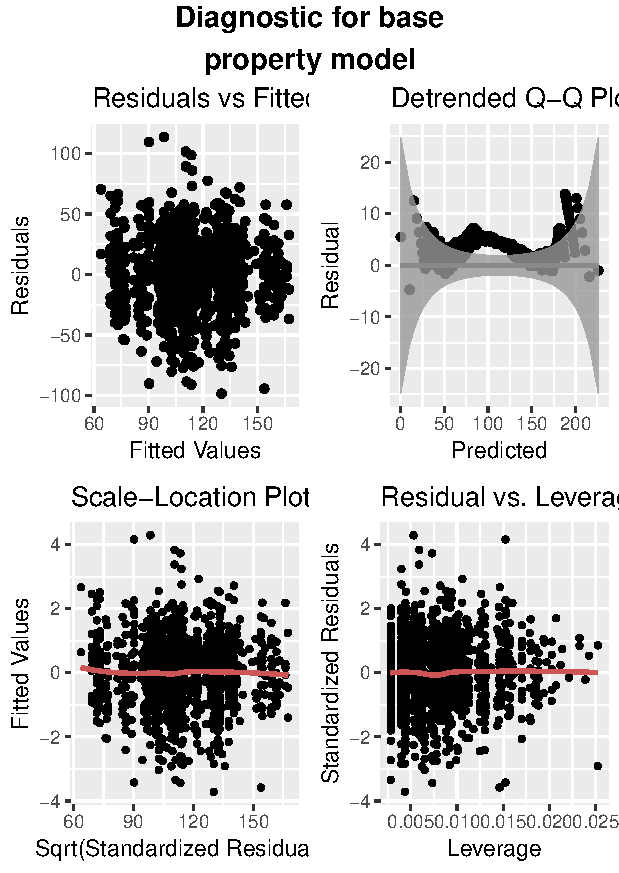
\includegraphics[width=0.4\textwidth]{diag_prop}
	\caption{Model diagnostic plots for our sub-models}
	\label{fig:smdiag}
\end{figure}

\section{Tables}

{ 
\begin{table}[H]
	\caption{Tables relating to model fit and variable independence}
	\begin{subtable}{0.45\linewidth}
		\footnotesize
		\centering
		\rowcolors{1}{white}{lgray}
		\begin{tabular}{r|llr}
			\hline
			& Variable 1 & Variable 2 & P-value \\ 
			\hline
			1 & Gas.cons & Age.band & 0.03 \\ 
			2 & Gas.cons & Type & 0.00 \\ 
			3 & Gas.cons & Floor.area & 0.00 \\ 
			4 & Gas.cons & Loft.depth & 0.55 \\ 
			5 & Gas.cons & Cavity.wall & 0.12 \\ 
			6 & Gas.cons & New.boiler & 0.31 \\ 
			7 & Age.band & Type & 0.00 \\ 
			8 & Age.band & Floor.area & 0.00 \\ 
			9 & Age.band & Loft.depth & 0.00 \\ 
			10 & Age.band & Cavity.wall & 0.00 \\ 
			11 & Age.band & New.boiler & 0.23 \\ 
			12 & Type & Floor.area & 0.00 \\ 
			13 & Type & Loft.depth & 0.72 \\ 
			14 & Type & Cavity.wall & 0.00 \\ 
			15 & Type & New.boiler & 0.16 \\ 
			16 & Floor.area & Loft.depth & 0.87 \\ 
			17 & Floor.area & Cavity.wall & 0.00 \\ 
			18 & Floor.area & New.boiler & 0.35 \\ 
			19 & Loft.depth & Cavity.wall & 0.68 \\ 
			20 & Loft.depth & New.boiler & 0.08 \\ 
			21 & Cavity.wall & New.boiler & 0.49 \\ 
			\hline
		\end{tabular}
	
		\vspace{0.5em}
		
		A p-value less than 0.05 means variables \\are (likely to be) statistically dependent.
		\caption{Table of results from Chi Squared test for independence. }
		\label{tab:chi}
	\end{subtable}
\begin{subtable}{0.45\linewidth}
	\footnotesize
	\centering
	\rowcolors{1}{white}{lgray}
	\begin{tabular}{r|lrr}
		\hline
		& Term & Estimate & Standard Error \\ 
		\hline
		1 & (Intercept) & 103.68 & 4.06 \\ 
		2 & Age.band2 & -0.96 & 2.37 \\ 
		3 & Age.band3 & -3.58 & 2.27 \\ 
		4 & Age.band4 & -4.84 & 2.34 \\ 
		5 & Age.band5 & -7.85 & 2.87 \\ 
		6 & Age.band6 & -13.76 & 2.95 \\ 
		7 & TypeDetached & 12.66 & 2.88 \\ 
		8 & TypeEnd-terrace & -5.97 & 2.74 \\ 
		9 & TypeFlat & -22.92 & 3.11 \\ 
		10 & TypeMid-terrace & -11.70 & 2.33 \\ 
		11 & TypeSemi-detached & 0.75 & 2.08 \\ 
		12 & Floor.area2 & 11.38 & 3.31 \\ 
		13 & Floor.area3 & 30.27 & 3.62 \\ 
		14 & Floor.area4 & 52.56 & 4.56 \\ 
		15 & Loft.depthLe & 1.98 & 1.98 \\ 
		16 & Cavity.wallY & -0.09 & 1.31 \\ 
		17 & New.boilerY & -2.78 & 1.34 \\ 
		\hline
	\end{tabular}
	\caption{Table of regression coefficients for the full model.}
	\label{tab:fulmo}
\end{subtable}

\end{table}

\begin{table}[H]

\end{table}
\end{document}